\graphicspath{{./figures}}

\section{Tracking and Pointing}

\subsection{Open-Loop}

In order to test the GPS pointing and open-loop tracking, a map was printed with lines pointing to nearby locations, from a pre-determined location as the origin. The ground station was then placed on top of this map at this location, and positioned to face magnetic north using a compass. This test had multiple goals i.e. to simultaneously test the mount transfer function, the GPS co-ordinate pointing, and the flight path data tracking. An image of the test setup is shown in Figure \ref{fig:pointingTest}.

\begin{figure}[!htb]
  \centering
  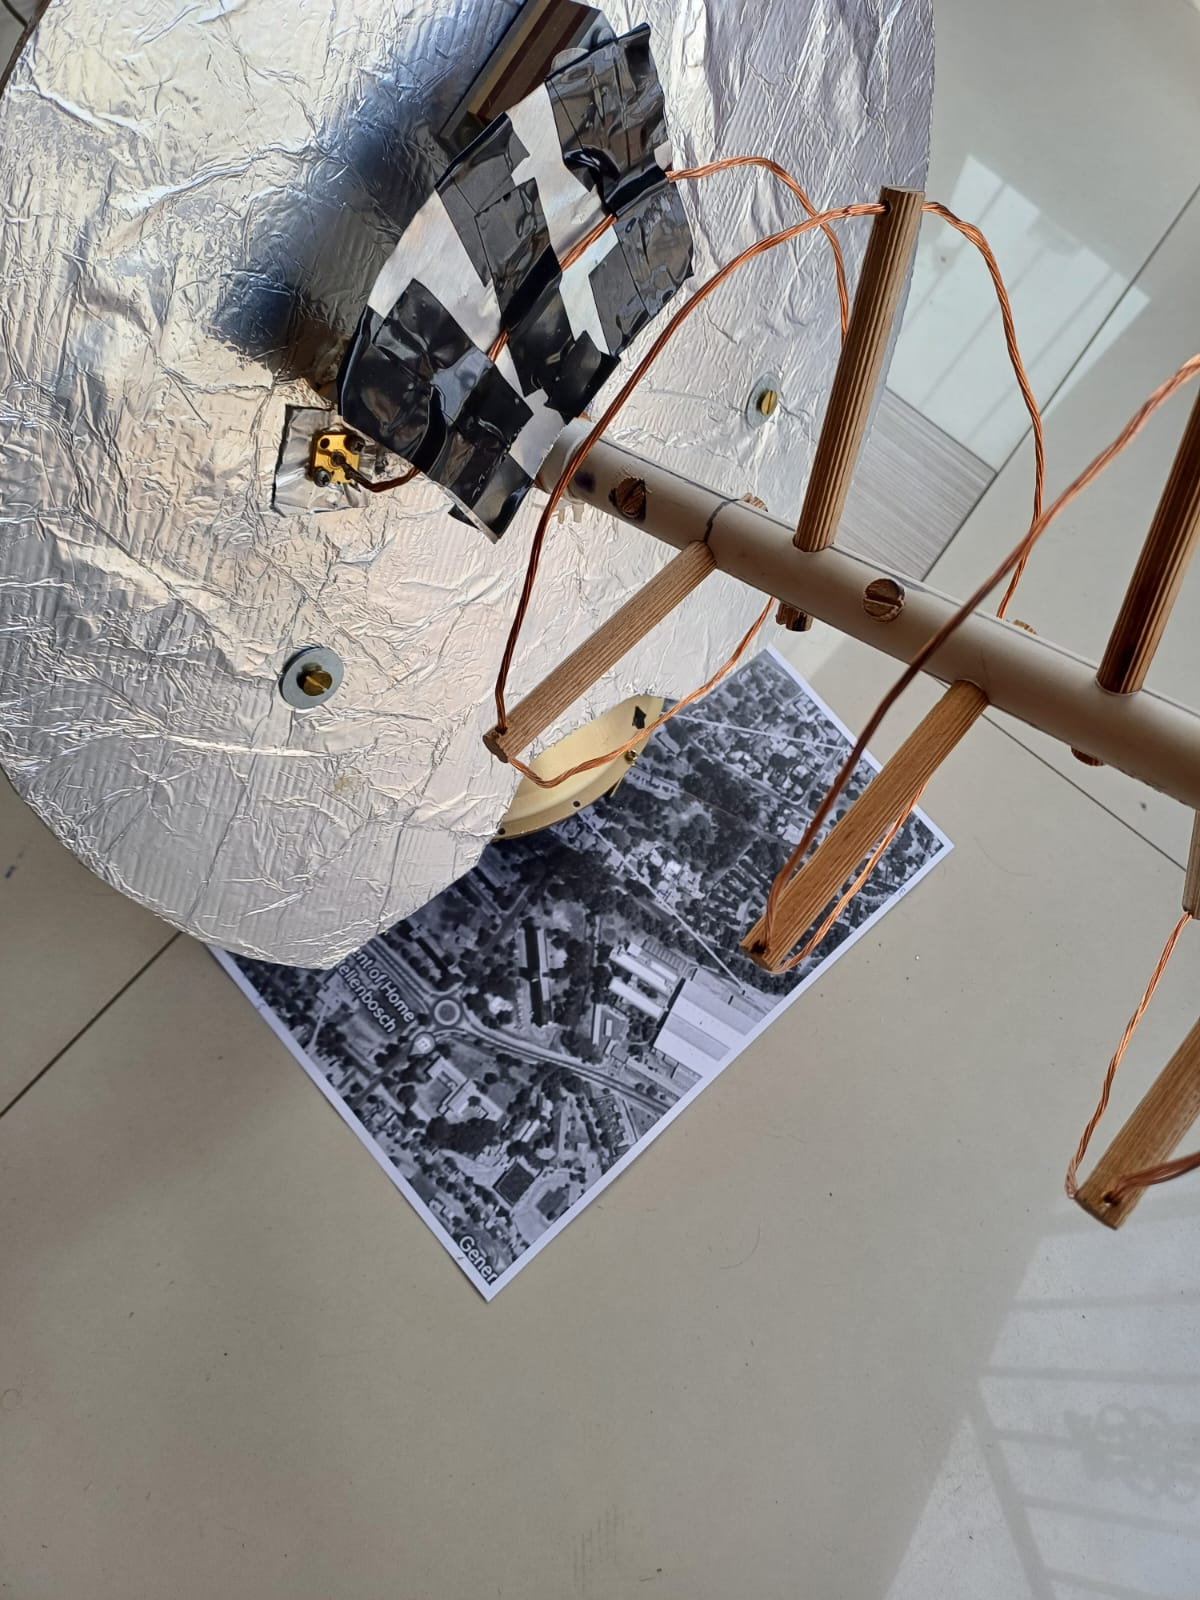
\includegraphics[width=0.4\textwidth]{pointingTestSetup}
  \caption{Pointing Test Setup}
  \label{fig:pointingTest}
\end{figure}

Flight path data containing the pre-determined co-ordinates was uploaded to the system, and the azimuthal angle was qualitatively confirmed to point in the directions labelled on the map using a ruler. Further, the elevation angle was measured using a protractor and compared against the expected angle. The system was found to successfully point towards the commanded locations at the desired times. The measured elevation angle was found to be within $5^\circ$ of the expected angle. This is considered to be within the limitations of the measurement system (the setup to measure the incline angle of the ground plane was non-ideal due to the bends in the ground plane and the awkward measurement procedure). Ideally, an accurate inclinometer should be used to confirm the elevation angles.

\subsection{Closed-Loop}

The closed-loop received location GPS tracking was tested on an open field with close to 300 m range. The PQ unit was carried around the field transmitting its GPS location, and the RSSI, as well as the antenna pointing direction, were recorded/observed.

\begin{figure}[!htb]
  \centering
  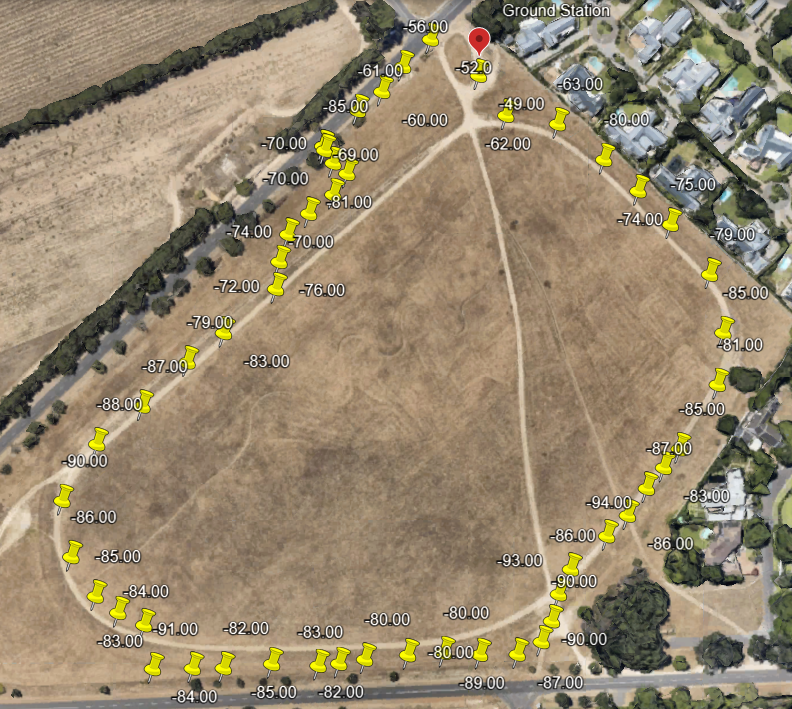
\includegraphics[width=0.6\textwidth]{gpsTrackingMap}
  \caption{GPS Tracking Locations and RSSI Values}
  \label{fig:gpsTrackingMap}
\end{figure}

The system was observed to successfully track the transmitter around the entire field without noticeable delay, until it reached a distance of around 10 m, where the pointing direction became unpredictable. This is attributed to the low accuracy of the GPS modules. Since the system is already known to have the capabilities of pointing at a GPS location (from the open-loop tests) and the time requirement is much lower for the balloon satellite system (which requires a tracking speed on the order of 45 degrees in an hour or two) it can be said that the system works as designed.

The above test also serves as a primitive test for GPS accuracy. The width of the main path being walked on was 3.2 m wide. The furthest mapped deviation of a received GPS co-ordinate from this path is measured at around 3 m (note that the map image is outdated). An upper bound on the GPS's accuracy can be therefore be said to be 6.2 m. Since the required accuracy for the system was calculated to be on the order of a thousand metres, it is clear that this meets the system requirements.